\documentclass{sigchi}

% Use this command to override the default ACM copyright statement
% (e.g. for preprints).  Consult the conference website for the
% camera-ready copyright statement.

%% EXAMPLE BEGIN -- HOW TO OVERRIDE THE DEFAULT COPYRIGHT STRIP -- (July 22, 2013 - Paul Baumann)
% \toappear{Permission to make digital or hard copies of all or part of this work for personal or classroom use is      granted without fee provided that copies are not made or distributed for profit or commercial advantage and that copies bear this notice and the full citation on the first page. Copyrights for components of this work owned by others than ACM must be honored. Abstracting with credit is permitted. To copy otherwise, or republish, to post on servers or to redistribute to lists, requires prior specific permission and/or a fee. Request permissions from permissions@acm.org. \\
% {\emph{CHI'14}}, April 26--May 1, 2014, Toronto, Canada. \\
% Copyright \copyright~2014 ACM ISBN/14/04...\$15.00. \\
% DOI string from ACM form confirmation}
%% EXAMPLE END -- HOW TO OVERRIDE THE DEFAULT COPYRIGHT STRIP -- (July 22, 2013 - Paul Baumann)

% Arabic page numbers for submission.  Remove this line to eliminate
% page numbers for the camera ready copy
\pagenumbering{arabic}

% Load basic packages
\usepackage{balance}  % to better equalize the last page
\usepackage{graphics} % for EPS, load graphicx instead 
\usepackage[T1]{fontenc}
\usepackage{txfonts}
\usepackage{mathptmx}
\usepackage[pdftex]{hyperref}
\usepackage{color}
\usepackage{booktabs}
\usepackage{textcomp}
\usepackage[super]{nth}
\usepackage{array}
\usepackage{siunitx}
\usepackage{multirow}
\usepackage[sort, nocompress]{cite}

% Some optional stuff you might like/need.
\usepackage{microtype} % Improved Tracking and Kerning
% \usepackage[all]{hypcap}  % Fixes bug in hyperref caption linking
\usepackage{ccicons}  % Cite your images correctly!
% \usepackage[utf8]{inputenc} % for a UTF8 editor only

% If you want to use todo notes, marginpars etc. during creation of your draft document, you
% have to enable the "chi_draft" option for the document class. To do this, change the very first
% line to: "\documentclass[chi_draft]{sigchi}". You can then place todo notes by using the "\todo{...}"
% command. Make sure to disable the draft option again before submitting your final document.
\usepackage{todonotes}

% Paper metadata (use plain text, for PDF inclusion and later
% re-using, if desired).  Use \emtpyauthor when submitting for review
% so you remain anonymous.
\def\plaintitle{SIGCHI Conference Proceedings Format}
\def\plainauthor{First Author, Second Author, Third Author,
  Fourth Author, Fifth Author, Sixth Author}
\def\emptyauthor{}
\def\plainkeywords{Authors' choice; of terms; separated; by
  semicolons; include commas, within terms only; required.}
\def\plaingeneralterms{Documentation, Standardization}

% llt: Define a global style for URLs, rather that the default one
\makeatletter
\def\url@leostyle{%
  \@ifundefined{selectfont}{
    \def\UrlFont{\sf}
  }{
    \def\UrlFont{\small\bf\ttfamily}
  }}
\makeatother
\urlstyle{leo}

% To make various LaTeX processors do the right thing with page size.
\def\pprw{8.5in}
\def\pprh{11in}
\special{papersize=\pprw,\pprh}
\setlength{\paperwidth}{\pprw}
\setlength{\paperheight}{\pprh}
\setlength{\pdfpagewidth}{\pprw}
\setlength{\pdfpageheight}{\pprh}

% Make sure hyperref comes last of your loaded packages, to give it a
% fighting chance of not being over-written, since its job is to
% redefine many LaTeX commands.
\definecolor{linkColor}{RGB}{6,125,233}
\hypersetup{%
  pdftitle={\plaintitle},
% Use \plainauthor for final version.
%  pdfauthor={\plainauthor},
  pdfauthor={\emptyauthor},
  pdfkeywords={\plainkeywords},
  bookmarksnumbered,
  pdfstartview={FitH},
  colorlinks,
  citecolor=black,
  filecolor=black,
  linkcolor=black,
  urlcolor=linkColor,
  breaklinks=true,
}

% create a shortcut to typeset table headings
% \newcommand\tabhead[1]{\small\textbf{#1}}

% End of preamble. Here it comes the document.
\begin{document}

\title{\plaintitle}

\numberofauthors{3}
\author{%
  \alignauthor{Leave Authors Anonymous\\
    \affaddr{for Submission}\\
    \affaddr{City, Country}\\
    \email{e-mail address}}\\
  \alignauthor{Leave Authors Anonymous\\
    \affaddr{for Submission}\\
    \affaddr{City, Country}\\
    \email{e-mail address}}\\
  \alignauthor{Leave Authors Anonymous\\
    \affaddr{for Submission}\\
    \affaddr{City, Country}\\
    \email{e-mail address}}\\
}



\maketitle
\begin{abstract}
This paper demonstrates advantages of measuring pupil fluctuation for recognizing cognitive load. Instantaneous heart rate, pulse transit time, heart rate variability, and Galvanic skin response were not good predictors of task difficulty for an overloaded driver experiencing complex sensory motor coordination with notifications.  Pupil fluctuation, on the other hand, was over 80 percent correct at distinguishing low and high task load  within 5 seconds. The paper presents a database with high and low task load regions that can be used by researchers for training across a variety of sensors for task load examination.  
A second experiment is presented which productively tracks high and low driving task loads with a pupil dilation model.  
Further work can easily improve the evaluation of high task load onset by modeling its rise and fall. The final experiment shows that the effect was present even during the day in a car. The paper introduces the pupil dilation model at a time when cameras and evaluation of pupils allow this new method to be used broadly.


%The real time factor becomes particularly important for dialog systems and other mixed-initiative interfaces.

\end{abstract}

% A category with the (minimum) three required fields
\category{H.5.m.}{Information Interfaces and Presentation (e.g. HCI)}{Miscellaneous}
%A category including the fourth, optional field follows...
% \category{D.2.8}{Software Engineering}{Metrics}[complexity measures, performance measures]

% \terms{Theory}

\keywords{Cognitive Load; Divided Attention; Psychophysiological Measures; Pupil Dilation}

\section{Introduction}
When are people available to work or communicate? Ubiquitous computing platforms like the mobile phone have become the gateway through which people access information and interact with others, in social and even physically engaged situations. The trend in technology can now  flip the paradigm and proactively provide information to the user. People, however, have a finite mental resource and can only process a limited amount of information without degradation of task performance. For cognitively challenging activities like driving, or even timing sensitive conversations like auctions or playing cards for money, divided attention can have dire consequences. Thus, there is a need for systems to gauge the load on this mental resource in order to predict or preempt degradation in task performance, while interacting with a user.

While progress has been made towards gauging this load, we are still a long way off from being able measure it in anything like a real time fine-grained level~\ref{todo}. In the future such capabilities might reduce task load to avert human mistakes. For instance, as speech technologies get better, voice interaction might be the most efficient way to interact with the user, when the user's manual and visual resources are occupied. A rapid and fine-grained measure would allow a dialog or proactive agent to track in real time the ebbs and flows of the load being experienced by the user. This would allow it to preempt disfluencies and other irregularities in speech, as well as to time its responses and other actions, so as to prevent overloading the user. In the driving scenario, its been shown that passengers adapt their conversation to task load, which leaves the driver with more resources to perform the driving task when it gets difficult~\cite{drews2008, cohen2014}. Interactive agents should aim to emulate such considerate behaviors.

This problem might be addressed by directly modelling the driver via psychophysiological measures, or by modelling driving context and its effect on the driver, or by jointly modelling both. Compared to modelling the driving context, less progress has been made in modelling the driver in order to identify when to interrupt them, or in factoring in the load from multitasking~\cite{kim2015}. One advantage of pursuing such an approach of modelling the user's internal state is the potential for these models to generalize to other domains, apart from driving. On the other hand, methods based on modelling situational context require specific sensors and modelling techniques to be considered for each domain separately. Furthermore, a psychophysiology-based approach can be tuned for each user individually, as different users might experience varying loads in a given situation. While costs and intrusiveness have stymied their widespread adoption, recent advances in wearable technologies suggest that monitoring at least a few physiological signals in everyday life might become a feasible option.

In this paper, we evaluate several signals that might be used in a psychophysiological approach to gauging user load while engaged in high task load and multitasking experiments. We wanted to capture the temporal aspects of divided attention --- the transitions in load when addressing and recovering from interruptions, for example. At the same time, we wanted to facilitate data collection that was repeatable with performance measures of a resolution suitable for real time task load evaluation or mediation. To meet these goals, we designed a driving-like primary task, with an intermittent secondary task of attending to and responding to notifications. As part of our initial explorations, we present results from two separate user studies. First, we created models that can detect which tasks the user is engaged in based on measurements of pupil dilation. We show how the performance of the model varies by changing the modality and timing of the notifications. We do this for each user, as well as across all users. Second, we built a real-time load detector based on pupil dilation measures, and used it to mediate notifications as part of a second user study. To the best of our knowledge, this is the first demonstration that pupil size variation can recognize and mark real time changes in task load. We present evaluations of the performance of the real time load detector, and the effect of its mediation on user task performance. 
\section{Related Work}
In cognitive psychology, there is a general consensus that people have limited and measurable cognitive capacities for performing mental tasks~\cite{miller1956}. Furthermore, engaging in one mental task interferes with the ability to engage in other tasks, and can result in reduced performance on some or all of the tasks as a consequence~\cite{kahneman1973}. To characterize the demand on these limited resources, psychologists have employed notions like cognitive load and mental workload, which gains definition through the experimental methods that are used to measure it \cite{klingner2010}. 

\subsection{Measuring Cognitive Load}
Cognitive load can be assessed using data gathered from three empirical methods: subjective data using rating scales, performance data using primary and secondary task techniques, and psychophysiological data from sensors~\cite{paas2003}. Self-ratings, being post-hoc and subjective in nature, make them inacurate and impractical to use when automated and immediate assessment is required. Secondary task techniques are based on the assumption that performance on a secondary measure reflects the level of cognitive load imposed by a primary task. A secondary task can be as simple as detecting a visual or auditory signal, and can be measured in terms of reaction time, accuracy, and error rate. However, in contexts where the secondary task interferes with the primary task, physiological proxies that can measure gross reaction to task load are needed to assess cognitive load.

\subsubsection{Psychophysiological Measures}
Psychophysiological techniques are based on the assumption that changes in cognitive functioning cause physiological changes. An increase in cortical activity causes a brief, small autonomic nervous response, which is reflected in signals such as heart rate (HR) and heart rate variability (HRV)~\cite{fredericks2005, mulder1992, wilson2002}, electroencephalogram (EEG)~\cite{ryu2005, wilson2002}, electrocardiogram (ECG)~\cite{ryu2005}, electrodermal activity (EDA)~\cite{ikehara2005, shi2007}, respiration~\cite{mulder1992}, and heat flux~\cite{haapalainen2010},eye movements and blink interval~\cite{beatty2000, ikehara2005, iqbal2005, wilson2002} pupillary dilations. Our dataset includes most of these signals as well as additional signals that have been shown to be sensitive to affect like pulse transit time (PTT), facial electromyography (EMG) and skin temperature~\cite{liu2008, or2007}. 

In this work strivesto correlate the effects of several physiological measures of cognitive function simultaneously in a multisensory motor scenario . In particular, brain activity as measured through event-related potentials using EEG, or as inferred from pupillary responses have received more attention recently because of their high sensitivity and low latency~\cite{antonenko2010, marshall2007, klingner2010}. There has been very little work that correlates these measures with the other physiological measures, or demonstrates how to effectively align them. Furthermore, to the best of our knowledge this is the only work that has focused on tracking cognitive load that is rapidly and randomly changing, since we are interested in teasing out the dynamic nature of instantaneous cognitive load.  Lastly, typical work has focuses on cognitive load arising in single-task scenarios like document editing~\cite{iqbal2005}, and traffic control management~\cite{shi2007}. In contrast, we employ a multitasking scenario, aspects of which we briefly review below.

%Leaving out the rest periods, which is usually employed between low and high control conditions allows us to capture the temporal patterns in these signals as they transition from low to high workloads, and vice versa.

\subsection{Multitasking Scenarios}
In multitasking scenarios, the distribution of cognitive resources when engaged in two or more tasks is not very well understood. This makes it difficult to assess and predict workload that will be experienced by the user. Theories have been proposed to model how multiple tasks might compete for the same information processing resources~\cite{wickens2008, baddeley2003}. One widely used approach that has been shown to fit data from multitask studies is Wicken's multiple resource theory. This attempts to characterize the potential interference between multiple tasks in terms of dimensions of stages (perceptual and cognitive vs. spatial), sensory modalities (visual vs. auditory), codes (visual vs. spatial), and visual channels (focal vs. ambient)~\cite{wickens2008}. Performance will deteriorate when demand for one or more tasks along a particular dimension exceeds capacity. 

In the case of driving and notification comprehension, both tasks compete for resources along the stages dimension. We would expect performance to deteriorate when there is an increased demand for the shared perceptual resources, i.e. when driving is hard and/or when the notification is difficult to comprehend. If the notification is visual, both tasks might also compete along the modality and visual channel dimensions. We would expect performance deterioration to be greater for visual notifications. 

\subsubsection{Driving and Language}
Listening and responding to another person while driving a car has been widely studied, and has been shown to effect driving performance, particularly with remote conversants~\cite{kubose2006}. Passengers sitting next to a driver are able to adapt their conversation to the traffic situation, allowing the driver to focus on driving when it becomes difficult~\cite{drews2008, cohen2014}. These findings have motivated research towards building dialog systems that are situation-aware and interrupts itself when required~\cite{kousidis2014}. As mentioned earlier, the focus in most of this work is on monitoring the driving environment, and less on determining the cognitive load of the driver. Recently, there has been an interest in studying the effect that complex linguistic processing can have on driving using physiological measures of pupil dilation and skin conductance~\cite{demberg2013}. 


\section{Study 1: Model Building}
The appeal of real world scenario is transfer of results. But such experiments suffer from lack of repeatability and reproducibility because of the large number of variables involved. Repeating a route, introduces learnable landmarks that change performance.  Events of interest happen unpredictably and infrequently. Establishing ground truth in such cases is also non-trivial and sometimes requires manual effort like scoring or annotating video recordings, etc. Experiments in the lab can circumvent a lot of these shortcomings by abstracting out the problem. A common practice in psychophysiology, however, is to have a control condition, followed by a test condition, with a rest period in between. As a consequence, the temporal aspects of psychophysiological signals as they fluctuate, is lost. 

% by allowing researchers to abstract out the problem and focus only on the particular aspects of it that are of interest to them

In collecting this dataset, we wanted the advantage of the lab setting, while still grappling with some of the complexity of real world data. In particular, we wanted to capture the temporal aspects of fluctuating psychophysiological signals while a participant is intermittently multitasking. We settled on an driving like primary task scenario. Attending and responding to notifications is a  secondary task. These two tasks allow investigation of the impact that the timing and modality of the notification would have on the load experienced by the user. 

Our goals with this dataset are to:
\begin{itemize}
\item Experiment with building models that can rapidly track cognitive load in a multitasking driving scenario
\item Study the impact that the timing and modality of an intermittent secondary task has on cognitive load
\end{itemize}

A user study using a driving simulator varied task load,  timing (mediated vs. non-mediated) and modality (audio vs. visual) of notifications being sent to the driver, while they performed the primary sensory motor steering and reaction tasks. The study was setup so that the driving task would randomly switch between low and high workloads. In the mediated condition, the audio notifications would be sent only during the low driving workload condition, in contrast to their random delivery in the non-mediated condition. With regards to modality, audio notifications were delivered via speakers, and visual notifications through Google Glass (Glass). Glass's optics projects the screen at a working distance of 3.5 m, approximately \SI{35}{\degree} elevated from the primary position of the eye. The audio notifications were created using Apple's text-to-speech engine on OS X Yosemite (Speaking voice: Alex; Speaking rate: Normal).



\subsection{Design}
The study was designed as a 2 (Audio/Visual modes) X 2 (Mediated/Non-mediated conditions) repeated measures within subjects study. To control for possible effects of order the study was double counterbalanced for the ?? mode and condition ??factors. Additionally, there was a baseline for each of low and high driving workload conditions. 

\subsection{Participants}
20 people (10 male, 10 female) participated in our study, recruited through a call sent out to students selected randomly from a graduate school population. The mean age of the participants was 26.4 years, with a standard deviation of 2.7 years. Participants were rewarded with a \$40 gift cards for completing the study.

\subsection{Tasks}
A multitasking scenario using a modified driving simulator created a random sequence of high and low workload periods. We elaborate below on the design of the primary driving task, and the secondary notification task.

\begin{figure}
\centering
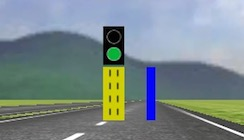
\includegraphics[scale=.8]{sim}
\caption{Screenshot of the ConTRe Task that displays the yellow reference cylinder with the traffic light on top, and the blue tracking cylinder.}
\label{fig:my_label}
\end{figure}

\subsubsection{Primary Task: Driving}
The primary driving task was implemented as the validated  of ConTRe (Continous Tracking and Reaction), which comes as an add-on for OpenDS, an open-source driving simulator~\cite{mahr2012}.  In ConTRe, the driver's task is comprised of steering and reactions to signals that mimic normal driving: operating the brake and acceleration pedals, and using the steering wheel. It differs from normal driving in terms of system feedback. Here the car moves autonomously with a constant speed on a unidirectional straight road consisting of two lanes. Operating the pedals or steering wheel has no effect on changing the speed or direction of the vehicle. Instead, these controls are used to manipulate a laterally moving cylinder, which is rendered in front of the car. 

The simulator shows two cylinders at a constant distance in front of the car: a yellow reference cylinder, and a blue tracking cylinder. The yellow reference cylinder moves autonomously according to an algorithm whose parameters can be set programmatically. The lateral position of the blue tracking cylinder is controlled by the driver through the use of the steering wheel. The cylinder moves left or right depending on the direction and angular velocity of the steering wheel, i.e the steering wheel controls the cylinder's lateral acceleration. The Subject's goal is to track the yellow reference cylinder, by overlapping it with the user-controlled blue cylinder, as closely as possible. This roughly mimics a steering task where the user has to follow a curvy road. A green light below and a red light above mimic a streetlight reaction task  placed on top of the yellow reference cylinder. At any time, neither of the lights or only one is turned on. The red light requires that the driver respond by depressing the brake pedal, while the green light corresponds to the accelerator pedal. As soon as the user reacts to the light by depressing the right pedal, the light turns off.

For the low and high driving workload, the lateral speed of the reference cylinder was set to values that were empirically determined to cause significant differences in driving performance measures. In the experimental conditions, the lateral speed of the reference cylinder was set to psuedorandomly shift between the low and high workload settings. For every shift, the duration of each workload was randomly set by the algorithm, and was programmed to be within specified intervals. 

\subsubsection{Secondary Task: Notifications}
The notification task was based on widely used measures of working memory capacity, which include operation span and reading span tasks~\cite{conway2005}. Working memory has been purported to be involved in a wide range of complex cognitive behaviors, such as comprehension, reasoning, and problem solving as it is thought to reflect primarily domain-general, executive attention demands of the task~\cite{engle2002}. In this work we do not aim to measure working memory per se, but instead want to measure the effect of engaging in a complex cognitive secondary task. Thus, we modify the span tasks for our purposes as described below.

In each condition, Subjects were presented with a series of twenty items, which included ten equations and ten sentences (see Table~\ref{table:span}). The math and sentence notifications were randomly interspersed, so as to prevent the driver from getting into a rhythm of expecting either one. After the driver had read or listened to each item, they indicated its veracity by verbally responding \textit{true} or \textit{false}. Sentences are `true' when they are sensically valid. 

After each item, the subject was presented with an isolated letter. After two, three or four items, the driving task was paused, and they were asked to recall the letters in sequence. This was done to mimic the behavior of drivers who usually attend to notifications while driving, and respond to them, or perform other tasks that require more attention, when stopped at a light, or while driving down a road with no noticeable gradient or curve at a constant speed~\cite{kim2015}. 

\renewcommand{\arraystretch}{1.3}
\begin{table} \centering
\begin{tabular}{@{}ll@{}}\toprule
\textbf{Type} & \textbf{Notification} \\ \midrule 
Math & $2/2 + 1 = 1$ \\ 
Sentence & \multirow{2}{5cm}{After yelling at the game, I knew I would have a tall voice}  \\ & \\
% & \\
\bottomrule
\end{tabular}
\caption{Examples of the two types of notifications }
\label{table:span}
\end{table}


% \subsubsection{Mediation}
% In this work, mediation was primarily involved with the timing of the notifications. In the non-mediated condition, the notification would be displayed on the Glass, or played over speakers at random intervals. In the mediated condition, the bounded deferral technique~\cite{horwitz2005} was used, where the notifications would be delayed while the driver was in a high workload setting. The notification would then be delivered a few seconds into the low workload setting. Mediation timing was chosen by an experimentor   could determine when to deliver the intervention message. If it was the case that a notification had been delivered, and the workload setting changed from low to high before the driver responded, there were different options depending on the modality. For the audio mode, the notification could be paused and continued at the next low workload period, or simply repeated. In the visual mode, the notification could be hidden till the next low workload period, when it would become visible again. The overall goal was not to overload the driver. The experimentor was tasked with using their intuition and judgement to avail of the different options, given the situation.

% Before each condition, participants were told which mode of notification they would be receiving, i.e.\ audio or visual. However, they did not receive any indication as to whether the notifications would be mediated or not. This was to test whether they would notice the shift in timing.

\subsection{Apparatus}
The Robot Operating System (ROS Hydro) was used to synchronize signals from the different components of the experimental setup. This included the simulator, physiological sensors, and the audio-visual feeds, all of which were running on different machines. Each component publishes messages via ROS Nodes to the server, which records the data as rosbags and writes it to disk. A Logitech camera along with mic and audio mixer was used to capture audio-visual information. Participants controlled the simulator using a Logitech G27 Racing Wheel.

\subsection{Physiological Sensors}
Physiological signals were captured and recorded using the Biopac's BioNomadix monitoring devices for ECG, Photoplethysmograph (PPG), EMG, Respiration, Skin Temperature, Electrodermal activity (EDA), and Impedance Cardiography (ICG). Pupil dilation and eye gaze was captured using Pupil Pro hardware\footnote{http://pupil-labs.com/pupil/}, which is a head mounted mobile eye tracking platform.

Since the hands of the participant were occupied for driving, we placed the PPG and EDA sensors on the participant's left toe \& instep, respectively~\cite{vanDooren2012}. The Facial EMG sensor was placed just above their left eyebrow to measure activation of the corrugator supercilii muscle, which is associated with frowning. Two skin temperature sensors were placed on the tip of the nose and on the left cheek. The ECG, impedance cardiography and respiration sensors were placed in the default positions, i.e. on the chest and neck. 

\subsection{Methodology}
Participants  were guided through an informed consent process, followed by an overview of the study. They were aided through the process of having a number of sensors attached to their body for the purposes of recording their physiological responses. The participant was then seated in the simulator and shown how notifications would be delivered on the Glass, and through binoral speakers. 

The dataset collection was split in two parts: baseline \& experimental. The baseline section records physiological measures for low and high driving workload separately. The experimental section records physiological measures for the multitasking scenario described in Section 3.3.  

\subsubsection{Baseline}
Each participant was taken through a series of practice runs to get them comfortable with the primary driving task. When done with the practice, the low benchmark was recorded using the low workload setting on the simulator. After a minute, they were asked to repeat a series of ten sentences that were read out to them, one-by-one, while they were still stearing and reacting to lights in the simulator. The same routine was performed to record the high benchmark using the high workload setting on the simulator. 

\subsubsection{Experimental}
This was followed by another set of practice rounds that combined both the driving task (with the randomly alternating workloads) and the notifications task. The notification task included a set of five items, three of which were equations, with the rest being sentences. This provided the participants with a sense of what to expect during the actual trials. The practice trials could be repeated if necessary. The participants then moved on to the experimental trials. Each participant had a total of four trials, one for each condition. The entire study lasted approximately 2 hours.





\subsection{Data Processing}


% \renewcommand{\arraystretch}{1.2}
% \begin{table*}[ht]
% \small
% \centering
% \begin{tabular}{|p{4.2cm} | p{3.7cm} | p{3.8cm} | p{3.4cm}|} \hline
% \multicolumn{2}{|c|}{\textbf{Physiological Measures}} & \multicolumn{2}{|c|}{\textbf{Performance Measures}} \\ \hline 
% \multicolumn{1}{|c|}{Raw} & \multicolumn{1}{|c|}{Derivative} & \multicolumn{1}{|c|}{Primary Task} & \multicolumn{1}{|c|}{Secondary Task} \\ \hline
% Electrocardiogram (ECG) & Pulse Transit Time (PTT) & Steering Deviation & Sentence Response Time \\ 
% Photoplethysmograph (PPG) & Inst. Heart Rate (IHR)} & Acceleration Reaction Time & Sentence Accuracy \\ 
% Impedance Cardiography(ICG) & SKT B $-$ SKT A (SKT) & Acceleration Accuracy & Math Response Time \\ 
% Respiration  & & Braking Reaction Time & Math Accuracy  \\ 
% Electrodermal Activity (EDA)  & &  Braking Accuracy & Recall Accuracy \\ 
% Skin Temp. Nose (SKT A) & &  & \\ 
% Skin Temp. Cheek (SKT B) & &  & \\ 
% Electromyography (EMG) & &  & \\ 
% Pupil Dilation  & &  & \\ 
% Eye Gaze &  &  & \\
% \hline\end{tabular}
% \caption{Collection of measures available in the dataset.}
% \label{table:measures}
% \end{table*}

\renewcommand{\arraystretch}{1.1}
\begin{table*}[ht]
\small
\centering
\begin{tabular} {@{}llcll@{}}\toprule
\multicolumn{2}{c}{\textbf{Physiological Measures}} &  \phantom{abc} & \multicolumn{2}{c}{\textbf{Performance Measures}} \\ 
\cmidrule{1-2} \cmidrule{4-5}
\multicolumn{1}{c}{Raw} & \multicolumn{1}{c}{Derivative} && \multicolumn{1}{c}{Primary Task} & \multicolumn{1}{c}{Secondary Task} \\ \midrule
Electrocardiogram (ECG) & Pulse Transit Time (PTT) && Steering Deviation & Sentence Response Time \\ 
Photoplethysmograph (PPG) & Inst. Heart Rate (IHR) && Acceleration Reaction Time & Sentence Accuracy \\ 
Impedance Cardiography(ICG) & SKT B $-$ SKT A (SKT) && Acceleration Accuracy & Math Response Time \\ 
Respiration  & && Braking Reaction Time & Math Accuracy  \\ 
Electrodermal Activity (EDA)  & &&  Braking Accuracy & Recall Accuracy \\ 
Skin Temp. Nose (SKT A) & &&  & \\ 
Skin Temp. Cheek (SKT B) & &&  & \\ 
Electromyography (EMG) & &&  & \\ 
Pupil Dilation  & &&  & \\ 
Eye Gaze &  &&  & \\
\bottomrule
\end{tabular}
\caption{Collection of measures available in the dataset.}
\label{table:measures}
\end{table*}


\begin{figure*}[th]
\centering
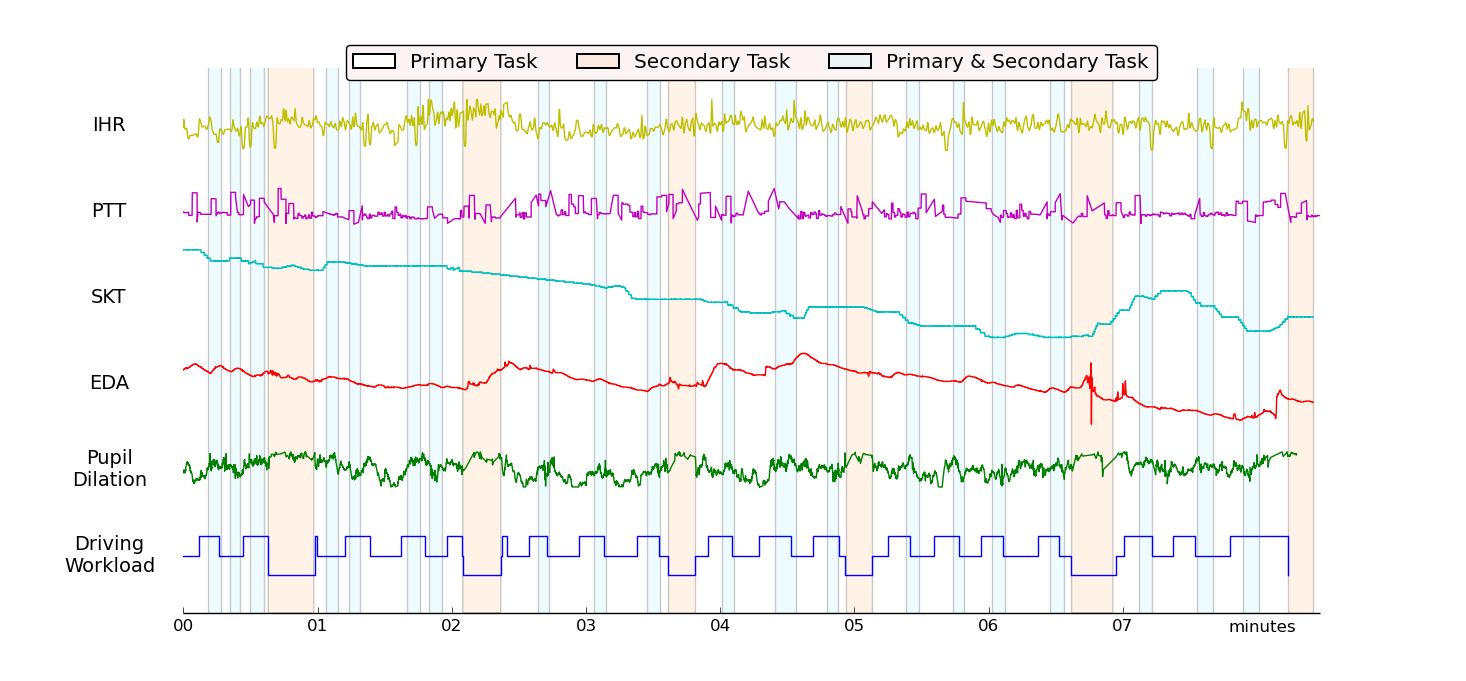
\includegraphics[height=8cm]{bwrepr}
\vspace{-1.5em}
\caption{Example physiological measures collected during an audio non-mediated experimental condition. Driving workload is represented as a step function (1: High, 0: Low, -1: Pause). Shaded regions delineate when the user was engaged in the primary driving task (P),  secondary notification task (S), or both (P \& S).}
\label{fig:snapshot}
\end{figure*}

The dataset consists of a number of physiological and performance measures which are tabulated in Table~\ref{table:measures}. We recorded ten psychophysiological signals: EDA, EMG, Skin temperatures (nose \& cheek), four signals based on cardiac activity (ECG, PPG, ICG \& Respiration), and two based on eye activity (gaze \& pupil dilation). Apart from the eye-based signals, which were sampled at 30 Hz, the rest of the signals were sampled at 2000 Hz. 

Three derivative signals were also calculated. Instantaneous heart rate (IHR) was obtained from the ECG signal using the BioSig library\footnote{http://biosig.sourceforge.net/} which implements Berger's algorithm~\cite{berger1986}). Pulse Transit Time (PTT) was obtained by calculating the difference in between the ECG R-wave peak time and the PPG peak time, which is the time it takes for the pulse pressure waveform to propagate through a length of the arterial tree. Difference in skin temperature (SKT) was also calculated by subtracting the temperature of the nose from that of the cheek.

The performance measures encompass both the primary driving task and the secondary notification task. Of interest are the reaction times and accuracies to the red and green light stimuli, and the steering deviation in tracking the reference cylinder. Also recorded are the performance measures for the secondary notification task as shown in Table~\ref{table:measures}.

\subsubsection{Preprocessing \& Labelling}
We analyzed the following five physiological signals: IHR, PTT, SKT, EDA and Pupil Dilation (Figure~\ref{fig:snapshot}). These signals were extracted from the rosbags and down-sampled to 40 Hz (except for pupil which remains at its original sampling rate of 30 Hz). Each signal was plotted, and thresholds were determined to filter out unlikely values (from movement artifacts, etc.). Data for each user was standardized (zero mean \& unit variance), prior to which outliers that were greater than three standard deviations were filtered out.

Two sets of labels are included in the dataset, one each for the primary and secondary task. By syncing with the timestamps from both the task logs, we determined the precise primary and secondary task conditions that the participant was under for every physiological sample. The primary task labels denotes if the participant is in the low, high or paused driving workload condition (see Driving Workload in Figure~\ref{fig:snapshot}). The logs from the secondary task allow us to determine the periods during which a participant was attending to a notification, i.e.\ blue regions in Figure~\ref{fig:snapshot}. The orange regions signify the recall part of the secondary task, when the primary driving task was paused.

\subsection{Feature Extraction}
We derived a number of statistical features on the main signal (x[n]), the derivative signal $(x[n+1] - x[n])$, and the percentage change $((x[n+1] - x[n])/x[n] * 100)$. These features include the mean, median, percentiles (\nth{10}, \nth{25}, \nth{75}, \nth{90}), ranges (between min and max, \nth{10} and \nth{90} percentiles, and \nth{25} and \nth{75} percentiles), skewness, standard deviation.

Features were extracted by moving a convolving data (3 to 7 datum) window across the signal. To capture some of the temporal properties, windows were overlapped by setting the step size to be smaller than the window size. Different window and step size lengths were considered. Specifically, the following pairs of window and step sizes (seconds) were analyzed: (7, 1), (5, 1), (3, 1) and (3, 0.25). 

\subsection{Modelling for Multitasking Scenario}
Based on the insights from Wilkin's multiple resource theory described in the section 2.2,  the primary and secondary tasks should no be not mutually exclusive, since resources along particular dimensions are shared. Thus, we can view this as a multilabel classification problem. In this formulation, each window is assigned two labels to denote the two possible tasks that the participant can be engaged in, for the duration of that window. For the purposes of this evaluation, the specific states of both tasks (low/high; attending/recall) are ignored reducing this to a multilabel binary classification problem. 

For the duration of the window, if the participant is only engaged in the primary driving task, the window is labelled as P. If the driving task is paused, and the participant is engaged in recall, the window is labelled as S. Since the duration of attending to a notification is usually shorter than 7 seconds, windows where a participant is attending to a notification for at least the first half while driving for the whole duration are labelled as both P and S. All other transitory windows were discarded.   

The features for each window, and the corresponding multilabel assigments \{P,S\} were fed to a Random Forest classifier, which is an ensemble technique that learns a number of decision tree classifiers and aggregates their results. Models were built across all users, as well as for each user separately, so as to account for individual differences in their psychophysiological response. To evaluate the classifier's performance, we used leave-one-user-out cross-validation for the population models, and 3-fold cross-validation for the individual user models. 

The time it takes to comprehend a notification varies by participant. This creates variation in the number of driving and notification task labels generated per participant, which in turn results in a varying baseline accuracy for each user. Hence, we report the area under  the Receiver Operating Characteristic (ROC) curve (AUC) instead of accuracy. ROC curves show the tradeoffs between higher sensitivity and higher specificity. Sensitivity refers to the correct detection of a condition or state when it is truly present. Specificity indicates the correct rejection of a state when it is truly not present. The area under the ROC curve is a measure of adequacy on both. Curves corresponding to random or chance classification of 50\% would fall close to the diagonal, and result in an ROC AUC score of 0.5, while the most successful classifications would have an ROC AUC score close to 1.0. 

Being a multilabel classification problem, the classifier outputs two probabilities simultaneously: one for the probability of the sample belonging to the primary task (P), and another for the probability that the sample belongs to the secondary task (S). We report the macro-averaged ROC AUC scores for the pair of labels, as a measure of how well the classifier is able to predict both labels (P, S). We also report the ROC AUC score for each label, individually, to shed light on how accurately the classifier is able to identify each task.

\subsection{Results}

\renewcommand{\arraystretch}{1.2}
\begin{table}[t]
\centering
\begin{tabular} {@{}ccrrrcrrr@{}}\toprule
\multirow{2}{*}{\parbox[c]{1.3cm}{\centering Window,\\Step (s)}} & \phantom{}
&  \multicolumn{3}{c}{Population} & \phantom{} & \multicolumn{3}{c}{Individual} \\
\cmidrule{3-5} \cmidrule{7-9}
%  && \multicolumn{1}{c}{P, S} & \multicolumn{1}{c}{P} & \multicolumn{1}{c}{S} && \multicolumn{1}{c}{P, S}& \multicolumn{1}{c}{P} & \multicolumn{1}{c}{S} \\
 && P, S & P & S && P, S & P & S\\
\midrule
7, 1 && 0.85 & 0.90 & 0.80 && 0.84 & 0.89 & 0.78 \\
5, 1 && 0.84 & 0.89 & 0.78 && 0.83 & 0.88 & 0.78 \\
3, 1 && 0.81 & 0.85 & 0.76 && 0.81 & 0.87 & 0.75 \\
3, 0.25 && 0.80 & 0.86 & 0.75 && 0.80 & 0.86 & 0.74 \\
\bottomrule
\end{tabular}
\caption{ROC AUC Scores for population and individual models using different window and step sizes}
\label{Tab:win}
\end{table}

For the four window and step size combinations considered, mean ROC AUC scores for the population and individual models are shown in Table~\ref{Tab:win}. A larger window size tends to provide better results, and this trend holds for both the individual and population models. The population scores are comparable to the average user scores, which tells us that the model based on pupil dilations is generalisable. 

Table~\ref{Tab:win} also shows ROC AUC scores for predicting each label individually. The scores indicate that the models are better at identifying when the user is engaged in the primary driving task (P) as compared to when the user is engaged in the secondary notification task (S). This might be because of the differences in load induced by equation and sentence notifications, and also from the differences in the notifications being right or wrong. Our model doesn't account for these yet, but each can be treated as a different class under the multilabel multiclass framework.


\begin{table}
\centering
\begin{tabular}{@{}rcrrr@{}}\toprule
Condition & \phantom{abc} & P, S & P & S\\
 \midrule
\multicolumn{1}{l}{\textit{Non-mediated \phantom{abcde}}} \\
 Video  && 0.88 & 0.90 & 0.86 \\
 Audio  && 0.90 & 0.92 & 0.88 \\
 Overall && 0.88 & 0.91 & 0.86 \\
\multicolumn{1}{l}{\textit{Mediated}} \\
 Video && 0.82 & 0.89 & 0.76 \\
 Audio && 0.81 & 0.88 & 0.74 \\
Overall && 0.81 & 0.89 & 0.74 \\
 \bottomrule
\end{tabular}
\caption{Population-based ROC AUC Scores under different timing and modality conditions.}
\label{Tab:NM}
\end{table}

We also compared how varying the independent variables of timing and modality impacted the ROC AUC scores. The results for these experiments are tabulated in Table~\ref{Tab:NM}. Only the analysis on the 7 second long windows are presented here as similar trends were observed for the other combinations. It is clear that mediating when notifications were sent, had a larger effect than modality, on the model's ability to identify the secondary task. To explain this, we must remember that in the mediated condition, the participant is sent notifications when they are in the low driving-workload state. Te multiple resource theory, projects that  the cognitive load on the user in this state is similar to the cognitive load they experience when they are in the high driving-workload state. Thus, there is an overlap between windows with and without the S label. In the non-mediated condition, this overlap is much smaller, as notifications are also delivered in the high driving-workload states. This allows the classifier to better identify the secondary task in the non-mediated condition.







\section{Study 2: Real-time Mediation}
The goal in this study was to use a real-time load classifier to mediate notifications to the user based on their task load. We modified the classification model that was built and analyzed in the previous study to work with streaming data. In particular, the model trained on data from the non-mediated condition with a window size of 5 seconds and step size of 1 second was used. Compared to the other window and step size pairs that were analyzed, this was the one that gave the most promising results during the pilot experiments.

The classifier reads input from the pupil dilation data stream and outputs a \{T1,T2\} classification every second. Since at this preliminary stage, we are only detecting what tasks the user is engaged in, we make the assumption that if the user is multitasking, i.e \{T1,T2\} = \{1,1\}, then the user is experiencing high load. In the future, we would like to be able to make more fine grained estimations about user load within each task (for example, T1 = 0, 1, 2, 3, etc., based on difficulty of the primary driving task).   

The experimental setup is similar to the one used in the previous study with some modifications to the design and tasks. These changes are described in detail below.

\subsection{Design}
Compared to the previous study, notifications were only presented using the audio modality. The study was designed as a repeated measures within subject study with only one independent variable, i.e. non-mediated (control) vs. mediated (test) conditions. To control for possible effects of order the study was counterbalanced. 

\subsection{Participants}
10 people (all male) participated in our study recruited through a call sent out to students selected randomly from a graduate school population.

\subsection{Tasks}
Since notifications are what the system needs to mediate, it cannot be used as the secondary task (T2) that the classifier detects. In this study a gear changing task is used instead as the secondary task. 
 

\subsubsection{Primary Task (T1): ConTRe}
The primary task remains the same as in the first user study. The participant has to track the yellow cylinder with the blue cylinder which is controlled via the steering wheel. The participant simultaneously has to respond to the red and green lights on the yellow cylinder by depressing the brake and accelerator pedals, respectively. The ConTRe task was set to alternate between periods of low and high workloads as described in the first study. 


\subsubsection{Secondary Task (T2): Gear Change}
A laptop screen is placed in front of the simulator such that its contents are easily visible below the yellow and blue cylinders presented on the simulator screen. Numbers from 1-6 are presented on the laptop screen, which correspond to the gears on the gear shifter which is included with the Logitech G27 Racing Wheel. The user was asked to shift to the right gear when the number changed on the screen. To create a high task load for the user, the gear number only changed when the ConTRe task was in its high load setting. The gear number was set to change every 1-3 seconds. 

\subsubsection{Mediated Task: Notifications}
The notification task is a simplified version of the one used in the previous study, where recall has been eliminated. The user is not presented with isolated letters that they are required to remember, and consequently the simulator is never paused. In this study, notifications only consist of math and sentence prompts that the user responds to with a true or false.  

\subsection{Apparatus and Sensors}
The apparatus used to conduct the experiment was the same as before. With regards to the physiological sensors, only the Pupil Pro headset was worn by the user as pupil dilation was the lone physiological measure of interest

\subsection{Methodology}
Participants were guided through an informed consent process, followed by an overview of the study. The participant was then seated in the simulator, and was asked to put on the Pupil Pro headset. They were instructed on how to perform the ConTRe task. Once comfortable with the task, the secondary gear change task was introduced. After this the math and sentence notifications were demonstrated to the user. Once the user was familiar with all the tasks the experimental trials were run. Each participant did two trials, one in which the notifications were mediated based on task load, and one in which they were not. 

Notifications were mediated by delaying them if they haven't started playing. If the user became loaded while a notification was playing, the notification would cut off and repeat itself when the user was not loaded. For better user experience, a trade-off had to be made between cutting off a notification, and confidence in the load detection. A trigger-happy system that cuts off a notification every time time a \{1,1\} is output by the classifier can be annoying to the user. Based on pilot studies, the protocol was set to delay or cut-off notifications anytime a series of either [\{1,1\}, \{1,1\}] or [\{1,1\}, \{1,0\}, \{1,1\}] classifications was output by the classifier. The system would then wait for a series of five \{1,0\} classifications before resuming delivery of notifications.  

\subsection{Measures}
Quantitative performance data on primary, secondary and mediated tasks were collected. From the primary ConTRe task, we collected the following: steering deviation, i.e. the difference in distance between the reference cylinder and the tracking cylinder (sampled at 570 Hz); reaction times to respond to the red and green lights, i.e. the amount of time from when the light went off to when the correct pedal was depressed; and the error rate of depressing the wrong pedal. These measures were automatically recorded by the simulator. Per user, there was an average of 13.7 and 23.8 acceleration stimulus points in the non-mediated and mediated conditions, respectively. Similarly, an average of 11.2 and 21.3 brake stimulus points were recorded in the non-mediated and mediated conditions, respectively. For each user in each condition, the mean steering deviation, reaction times and reaction errors were calculated.  

From the secondary gear changing task, the number of tries the user took to get to the right gear, and the number of times they didn't succeed are calculated. The mean of these measures for each user in both condition was also calculated. Per user, there was an average of 28.3 stimulus points in the non-mediated condition, and 52.2 stimulus points in the mediated condition. 

For performance on the mediated notification task, the response times for math and sentence prompts were computed. This is the time from when the notification was presented to the driver, to when they respond to indicate true or false. The mean response times for math and sentences are then recorded for each user in every condition. The errors in the responses, and the mean per user was also calculated for each condition. There was an average of 7.5 math and sentence prompts per user in each condition. 

The outputs from the classifier, which occur every second, were also recorded for the mediated condition. These will be analyzed to shed light on how the classifier's outputs could inform the systems mediation behavior.

\subsection{Results}
Below we report on results from the experiment. We look at mediation effects on each task by collectively analyzing their different measures. Since this presents three comparisons, we use the Bonferroni adjusted alpha levels of .017 per test (.05/3) to control for Type I errors. To perform the analysis for each task, we use a multivariate ANOVA (MANOVA) using their respective performance measures as dependent variables. As opposed to running multiple univariate F tests for each dependent variable, MANOVA has the advantage of reducing the likelihood of a Type I error, and revealing differences not discovered by ANOVA tests~\cite{warne2014}. We also analyze classifier performance to shed light on the trade-off between sensitivity and specificity.

\begin{table}
\centering
\begin{tabular}{@{}rcrrr@{}}\toprule
Performance Measures & \phantom{a} & M & N & \textit{p}\\
 \midrule
\multicolumn{1}{l}{\textit{Primary Contre Task \phantom{abcabcabc}}} \\
 Steering Deviation (\%)      && 22.0 & 23.1 & .47 \\
 Accel Reaction Time (ms)     && 980  & 1014 & .67 \\
 Brake Reaction Time (ms)     && 1117 & 1157 & .47 \\
 Accel Response Error Rate    && 0.34 & 0.23 & .07 \\
 Brake Response Error Rate    && 0.25 & 0.32 & \textbf{.05} \\
  \midrule
\multicolumn{1}{l}{\textit{Secondary Gear Task }} \\
 Attempts per stimulus        && 1.15 & 1.26 & \textbf{.015} \\
 Success Rate                 && 0.22 & 0.31 & \textbf{.05} \\
 \midrule
\multicolumn{1}{l}{\textit{Mediated Notification Task}} \\
 Math Reaction Time (s)       && 2.02 & 2.30 & .19 \\
 Sent. Reaction Time (s)      && 2.30 & 2.53 & .32 \\
 Math Response Error Rate     && 0.08 & 0.08 & .82 \\
 Sent. Response Error Rate    && 0.22 & 0.27 & .33 \\
 \bottomrule
\end{tabular}
\caption{Population-based ROC AUC Scores under different timing and modality conditions.}
\label{Tab:T123}
\end{table}

\subsubsection{Mediation Effects}
The analysis of mediation effect on the primary ConTRe task using a repeated measures MANOVA showed no significant effect, \textit{F}(5,5)=1.44, \textit{p}=.35. The means for each of the five primary task measures in both conditions, and the paired t-test two-tailed p-values are listed in Table~\ref{Tab:T123}.

For the secondary gear changing task, a repeated measures MANOVA showed a significant effect, \textit{F}(2,8)=7.42, \textit{p}=.015. Further analysis of each of the dependent variables showed a significant different in the mean number of tries the user took to get to the right gear between the mediated (\textit{M}=1.15, \textit{SD}=0.16) and non-mediated (\textit{M}=1.26, \textit{SD}=0.14) conditions, \textit{t}(9)=-3.72 , p=.004. There was also a slightly significant difference in the failure rates between the mediated (\textit{M}=0.22, \textit{SD}=0.05) and non-mediated (\textit{M}=0.31, \textit{SD}=0.13) conditions, \textit{t}(9)=-2.26 , p=.05. These are listed in Table~\ref{Tab:T123}.

A repeated measures MANOVA for the mediated notification task revealed no significant effect, \textit{F}(4,6)=0.98, \textit{p}=.48. The means for each of the four notification task measures in both conditions, and the paired t-test two-tailed p-values are listed in Table~\ref{Tab:T123}.

\begin{table}
\centering
\begin{tabular}{@{}rcrrr@{}}\toprule
System Stimulus & \phantom{a} & Sens. & Spec. & Acc.\\
 \midrule
 every \textit{H} and \textit{L} && 40 & 72 & 61 \\
 \textit{H} 
 && 90 & 19 & 56 \\
 \midrule
 \textit{HH} or \textit{HLH}
 && 83 & 42 & 63 \\
 \textit{HHH} 
 && 74 & 68 & 71 \\
 \textit{HHHH} 
 && 58 & 82 & 70 \\
%  \textit{HHHHHH}
%  && 46 & 89 & 67 \\

 \bottomrule
\end{tabular}
\caption{Population-based ROC AUC Scores under different timing and modality conditions.}
\label{Tab:Spec}
\end{table}

\subsubsection{Classifier Performance}
Since the classifications are done on a sliding window, we can expect a lag from the onset of high load to when the classifier output indicates so. Another reason for the delay in classifications might be that even though a high load is being imposed on the user, it might take a couple of seconds for them to experience it as such. By performing cross-correlation of time-shifted classification outputs with the alternating low and high load conditions that each user was subjected to, the time-shift at which the cross-correlations were maximum were determined. Across users, the average optimal time-shift was 4.9 seconds, with a standard deviation of 1.44. For further analysis, this number was rounded up, and the classification outputs were time-shifted by 5 seconds for each user. For simplicity, we represent a \{1,0\} classifier output as \textit{L} and a a \{1,1\} classifier output as \textit{H}. 

By being overly eager or overly cautious, a system can display two extremes in how it uses the classifier outputs to inform its mediation behavior. In case of the former, the system reacts immediately to every \textit{L} and \textit{H} being output by the classifier. We would expect the classifier to have high specificity, as it immediately corrects its behavior. In case of the latter, the system is very cautious about interrupting the user and reacts to the \textit{H} but ignores the \textit{L}. It is highly sensitive to an \textit{H} and immediately delays or cuts off a notification, even if the \textit{H} is followed by \textit{L}s. Thus it displays low specificity. For our evaluation purposes, we can view this extreme case as correct classification (true positive) if a single \textit{H} is detected during a high load section, and conversely, an incorrect classification (false positive) if a single one has been detected during the low load section. These two extremes are shown in Table~\ref{Tab:Spec}, along with a few intermediate behaviors which we describe next.

To trade-off between sensitivity and specificity, the system could be designed to respond only if it sees a particular set of patterns. A few example patterns were evaluated, and their results are listed in Table~\ref{Tab:Spec}. These include patterns such as [\textit{H},\textit{H}] or [\textit{H},\textit{L},\textit{H}] which reduces the sensitivity of the system to the classifier outputs, making it less cautious. We can reduce system sensitivity even further by designing the system to mediate notifications only when it sees [\textit{H},\textit{H},\textit{H}] or [\textit{H},\textit{H},\textit{L},\textit{H}] from the classifier. We evaluate one more set of patterns to further desensitize the system. As the corresponding accuracy begins to drop, we might choose to design the system to respond to the pattern corresponding to the highest accuracy as a satisfactory trade-off.  



\section{Discussion}
This study compiles a dataset of psychophysiological signals to estimate cognitive load.  The measurments included  Electrodermal Activity,MechanoMygram Electro, Skin temperatures, ElectroCardioGram , Photoplethysmoragraph, ImpedenceCariograph,  Respiration, gaze, and pupil dilation. Apart from the eye-based signals, which were sampled at 30 Hz, the rest of the signals were sampled at 2000 Hz. 
Deriviative signals of Instantaneous heartrate, Pulse Transit Time and Difference in Skin temperature are also calculated in the dataset. 

Three derivative signals were also calculated. Instantaneous heart rate (IHR) was obtained from the ECG signal using the BioSig library\footnote{http://biosig.sourceforge.net/} which implements Berger's algorithm~\cite{berger1986}). Pulse Transit Time (PTT) was obtained by calculating the difference in between the ECG R-wave peak time and the PPG peak time, which is the time it takes for the pulse pressure waveform to propagate through a length of the arterial tree. Difference in skin temperature (SKT) was also Heartate variabiliy, HeartrateSituations of divided attention are now commonplace due to technological advancements. 

The Primary and secondary tasks were created to be difficult enough to elicit significant errors when a secondsary task was added for high task load.  The task load is created by a primary senimotor steering/reaction task and a secondary verbal/cognitive task to satisfy: a) a multitasking scenario that balanced the need for realistic interactions, with the need for repeatability, and b) a dataset that captured the dynamic nature of cognitive load as reflected in the participants' physiological responses. To this end, we used the CoNTR driving like scenario, where the participant intermittently attended to notifications as a secondary task. We also modulated the timing and modality of the notifications to understand their effects on cognitive load. ??? reference for verbal tasks???

We cast the multitasking scenario as a multilabel learning problem, and assigned labels to the primary and secondary tasks. We evaluated the utility of this approach, and showed that we were able to to use machine learning to build models that distinguish whether the user is engaged in the primary task, the secondary task, or both. This was demonstrated for each user individually, and across all the participants. These models were built using a number of statistical features derived from measurements of pupil dilation, which were fed to a random forest classifier. Furthermore, our evaluation showed that compared to the modality of delivery, the timing of the notifications have a larger effect on the load experienced by the user while driving. 

To show that pupil size variation metrics can be robust we used inexpensive off the shelf measuring technique. Prior work report use of expensive eye-trackers with higher sampling rates for pupilometric measurements. Other eye-camera measures of blink rate and gaze activity were not included in this analysis. Our study succeeded with an off-the-shelf webcam (Microsoft LifeCam HD-6000) with a sampling rate of 30 Hz specially mounted to view the pupil.  Even when tested outdoors in a car during the day,  with no special attempt to control for ambient luminescence the system was effective at producing pupilary size variation measures (perhaps the standardization step at the data reprocessing stage reduced its effect). More work could be done to refine the setup and understand the trade-offs between the fidelity of the equipment, environmental setup, and the robustness of results. 

!!!!Results the data for pupil is explored in a comapgnion paper and shown to best the others... we could recognize high task load low task load onset!!!

\subsection{Future work}
There are a number of investigative ways to approach the dataset, and we discuss three here (response filtering, ground truth calibration, and modeling stress source and timecourse). The first is with regards to learning temporal models, which include transitions between cognitive states. In the fields of cognitive science and psychophysiology, task-evoked responses are used to make fine-grained measurements on cognitive load, whereas human-computer interaction researchers generally use aggregated measures over a period of time to obtain more coarse and robust measurements~\cite{klingner2008}. By using overlapping  data averaging windows and statistical features we have merged the two approaches. Task load change modelling would certainly be improved by include the transition states from low to high task load discarded for the analysis in this paper. Temporal models based on task load change instead of static task load would speed and futher improve robustness of our already good prediction based on a sequence of observed physiological measures.  

A second approach brings into question the ground truth of the cognitive load experienced by the users. One option would be to use the recorded reaction times, or some composite of the different task performance measures, as a high resolution measure of ground truth. These could be used to learn regression models on the psychophysiological signals. The idea here is that if we can predict reaction times, we can estimate at a fine-grained level the cognitive load being experienced by the user. Another option would be to use the pupil dilation measure as a ground truth.

A third approach is based on differentiating between cognitive load and short-term acute stress. While there are no doubts that they are related, its not clear how to measure them independently, and how one confounds the other. There is good consensus in the literature regarding conditions where stress is likely to arise --- failure at a task, together with feelings of lack of control, in situations where participants are evaluated by others~\cite{conway2013}. We might thus hypothesize that stress is an affect, which ebbs and flows at a slower pace than cognitive load which fluctuates more rapidly, reflecting the stages of mental processing. It is possible that some physiological signals are better indicators of stress than cognitive load, while some are sensitive to both. A first step would be to contrast the signals in the baseline condition with the experimental conditions. Signals with longer drag times might be more reflective of stress. A related step would be to correlate the different measures, and explore how to effectively align them to get a more complete picture of a user's mental and affective state. 

\section{Conclusion}
This paper presents a data set showing cognitive load changes across task load changes.  The tasks were created to be difficult enough to elicit significant errors when a secondsary task was added for high task load.   The measurments included  Electrodermal Activity,MechanoMygram Electro, Skin temperatures, ElectroCardioGram , Photoplethysmoragraph, ImpedenceCariograph,  Respiration, gaze, and pupil dilation. Apart from the eye-based signals, which were sampled at 30 Hz, the rest of the signals were sampled at 2000 Hz. 
Deriviative signals of Instantaneous heartrate, Pulse Transit Time and Difference in Skin temperature are also calculated in the dataset.
!!! below update with your new experimental result!!
The burden is on the technology to determine the appropriate time to engage the user. One approach to do this is to gauge the cognitive load of the user using psychophysiological signals. While prior work has made progress in identifying such measures, lots of work still needs to be done to understand how to track rapid fluctuations in cognitive load in real time, especially in multitasking scenarios. To address this, we created a dataset of physiological measures, collected from participants in a multitasking study where they attended and responded to notifications while driving. We also collected a number of corresponding performance measures on both tasks. As an initial undertaking, we built models using statistical features extracted from pupil dilation measures. We showed that the resulting population model is capable of identifying the tasks the user is engaged in with an ROC AUC score of 0.85.

This paper presents a database eliciting cognitive function change accross high and low task load comparing 11 different physiological measures of cognitive function.  The tasks were chosen to elicit enough work to cause all subjects to make significant errors in the highest load conditions. Our initial findings show new valuable metrics for temporal change of cognitive load. We hope these to inspire other reserachers to use our dataset and to produce more such comparatie datasets as well.  


Our initial findings from this dataset show presented in a companinon paper []show that pupilary size variation was the only reliable measure for task load traccking that could track task loads in the near realtime 5 second range.  Indeed, our experminatation indicates that while modelling task load change might improve our anaysisis and bring the variation specificity down to 3 seconds beyond that is likely below the physiolotical response time of we could find.  
Initial exploration also found that pupilary dialation measures could be found and measured inside a car in daylight conditions.  The work also includes a new dataset in which machine learning model  on pupilary dialation was able to track task load change with better than 80 percent reliability.

This paper then presents that pupilary dialiation measures can be taken cheeply and in the wild to directly measure task load level in complex and coordinated tasks accross sensory motor verbal accuuision and cognitive task requests.
We see cognitive load assement as a rich area that could greatly improve human performance in many ways.  By measureing task load's effect we can modulate the difficulty of tasks we attempt.  By measuing task load effect computers can know when to reduce stimulation notification task requrest of any kind.  We hope this work inspires others to develop task load sensitive tests and user  experiences as well.





\balance{}

%
% The following two commands are all you need in the
% initial runs of your .tex file to
% produce the bibliography for the citations in your paper.
\bibliographystyle{SIGCHI-Reference-Format}
\bibliography{sigproc}  % sigproc.bib is the name of the Bibliography in this case
% You must have a proper ".bib" file
%  and remember to run:
% latex bibtex latex latex
% to resolve all references
%
% ACM needs 'a single self-contained file'!
%

\end{document}
